\section{Results}
\label{sec:Results}

\fix{Need an intro paragraph}

\subsection{Experimental Setup}

All experiments were performed on the Cielo supercomputer housed at Los Alamos
National Laboratory.  Cielo is an 1,840-node Cray XE6 resource for the Advanced
Simulation and Computing (ASC) program and is jointly managed by Sandia National 
Laboratories and Los Alamos National Laboratories under the New Mexico
Alliance for Computing at Extreme Scale (ACES) project.  Each node contains
two AMD Opteron 6100 (Magny-Cours) 8-way processor chips for a total of 16 cores
per node.  Each core has a peak computational speed of 2.6 GHz, leading to a total 
theoretical peak of 1.37 Petaflops for the machine. The compute nodes each
have 32 GB of memory.  The interconnect consists of a proprietary Cray Gemini
Network with a 3D Torus topology and has a peak throughput rate of 6 GB/s/link. 

This report includes strong scaling results from the following CTH
applications:
\begin{description}

\item [\Insitu optimized:] A CTH application that performs \insitu analysis
using a scalable version of the CTH analysis algorithm. \fix{Nathan describe
this}.  

\item [\Insitu unoptimized:] A CTH application that uses the original version of the 
analysis algorithm to perform \insitu analysis.  \fix{Nathan describe this
algorithm.}   We included results from this application for two reasons: First,
we were not able to apply the same optimization to the \intransit applications,
so this provides an apples-to-apples comparison of the benefit an \intransit
approach could give using the same algorithm.  Second, we expect the complete
fragment detection algorithm to have scalability issues similar to this
algorithm. \fix{Ken, explain this... something to do with connectivity?}

\item [\Intransit using extra nodes:] A CTH application that performs \intransit analysis
using a separate allocation of compute nodes.  This represents a use case where there are 
additional compute nodes (perhaps with special OS, runtime, or hardware features) that
could be used to perform analysis on behalf of the application.   For example, the suggested
``burst buffer'' architecture for the Trinity system may have special nodes
with NVRAM and additional memory that would be appropriate for this type of
\intransit analysis. 

\item [\Intransit using internal nodes:] A CTH application that divides the nodes from a given
allocation into compute and analysis nodes.  We chose this application to find out if, 
given an equal number of resources for \insitu and \intransit, there might be
situations where the preferable approach changes.  

\item [Spyplot file] A CTH application that writes Spyplot files instead of doing 
analysis.  This application represents the traditional post-processing approach.
\end{description}

All applications complete 500 cycles (i.e., timestep calculations) of the CTH
code. The first four applications execute an analysis operation once every 10
cycles.  For the Spyplot file application, we output spyplot data at a fixed 
interval in simulated time, calculated so that the application executed 51
I/O operations, equaling the number of analysis operations performed by the
\insitu and \intransit applications.  We do not know of a way to tell CTH to
output spyplot data every 10 cycles. 


%%%%%%%%%%%%%%%%%%%%%% -- table ---
\begin{table}[htb]

\caption{Scaling Overview}
\label{tab:ScalingOverview}

\centering{}%
\begin{tabular}{|c|c|c|}
\hline 
Data Set Size (blocks) & Client Ranks (16 cores/node) & Server Nodes (2, 4, and 8 cores/node)\tabularnewline
\hline 
\hline 
33k & 128, 256, 512, 1024 & 2\tabularnewline
\hline 
220k & 1024, 2048, 4096, 8192 & 16\tabularnewline
\hline 
1.5m & 4096, 8192, 16384, 32768, 65536 & 128\tabularnewline
\hline 
\end{tabular}
\end{table}

%%%%%%%%%%%%%%%%%%%%%% -- table ---

For each application, we ran strong scaling experiments for three different datasets.  
Table~\ref{tab:ScalingOverview} shows the range of core sizes used for the various
experiments.  For every application we used the maximum 16 cores-per-node for the CTH client,
since CTH is primarily bound by computation and scales very well.  For the \intransit service, 
we experimented with different core-per-node counts to balance the memory requirements
with the computational requirements of the ParaView analysis. 

%The objective is run experiments with datasets representative of real
%production runs.  The minimum number of cores per dataset is limited by
%memory.  The maximum number of cores per dataset was decided to get scaling data,


\subsection{Total Execution Time}
\label{tab:ScalingOverview}

\fix{more discussion}

\begin{figure*}[htb]
\begin{centering}
\vspace{-6pt}
\subfloat[\Insitu Unoptimized.]{
  \includegraphics[width=0.5\linewidth]{figures/in-situ-unopt-line}
  \label{fig:cth-in-situ}
}
\subfloat[\Insitu Optimized.]{
  \includegraphics[width=0.5\linewidth]{figures/in-situ-opt-line}
  \label{fig:cth-in-transit}
}

\vspace{-6pt}
\subfloat[\Intransit with extra nodes.]{
  \includegraphics[width=0.5\linewidth]{figures/in-transit-extra-line}
  \label{fig:cth-in-transit}
}
\subfloat[\Intransit using internal nodes.]{
  \includegraphics[width=0.5\linewidth]{figures/in-transit-inclusive-line}
  \label{fig:cth-in-transit}
}

\vspace{-6pt}
\subfloat[Spyplot I/O (no analysis)]{
  \includegraphics[width=0.5\linewidth]{figures/spyplot-file-line}
  \label{fig:cth-in-transit}
}
\caption[]{Total runtime for 500-cycle runs of each application.}
\label{fig:runtime-individual}
\end{centering}
\end{figure*}

Figures~\ref{fig:runtime-individual}~and~\ref{fig:runtime-total} shows the
measured total execution time from each the different applications. 
The first set of plots shows individual timings of each of the applications for each 
size dataset, the second shows a direct comparison of all the applications for 
the 1.5m block data set.  The results clearly show a ``sweet spot'' at 8K cores where
the \intransit approach, even though it is using a less scalable algorithm,
performs the same as the the optimized version of \insitu.   At 16K and 32K, none
of the codes running analysis show significant improvement, the unoptimized \insitu and the
\intransit approaches actually take longer.  Perhaps the biggest reason is that there
is not enough work for the compute nodes.  At 32K cores, each core is processing around 
46 blocks/node, where the same size problem using 4K nodes requires each core to process 
366 blocks.  The key to making the \intransit approach successful is being able to 
overlap computation and analysis.   If the analysis portion does not scale particularly
well, the compute nodes need sufficient work to hide the analysis cost. 

\begin{figure}[htb]
\begin{centering}
\includegraphics[scale=0.7]{figures/total-runtime-all.pdf}
\caption{Execution time comparison for the 1.5m block dataset.}
\label{fig:runtime-total}
\par\end{centering}
\end{figure}

To better understand exactly where the time is being spent, we collected
detailed timings of each application using a combination of instrumented timers
and profiling tools (HPCToolkit).  Figure~\ref{fig:runtime-individual-bar} show
the total runtime performance of the five applications as a stacked barplot
illustrating the portion of runtime associated with select functions.  For the
\insitu applications, we measured the initialization and computational time of
CTH and the analysis/visualization.  For \intransit applications, we measured
the initialization cost of CTH, the cost of transferring data to the service,
and the time the client waits for the server operation to complete. The wait
only occurs after CTH has finished its operation only executes if the 

\begin{figure*}[htb]
\begin{centering}
\vspace{-24pt}
\subfloat[\Insitu Unoptimized.]{
  \includegraphics[width=0.5\linewidth]{figures/in-situ-unopt-bar}
  \label{fig:insitu_unopt_bar}
}
\subfloat[\Insitu Optimized.]{
  \includegraphics[width=0.5\linewidth]{figures/in-situ-opt-bar}
  \label{fig:insitu-opt-bar}
}

\vspace{-24pt}
\subfloat[\Intransit with extra nodes.]{
  \includegraphics[width=0.5\linewidth]{figures/in-transit-extra-bar}
  \label{fig:intransit-extra-bar}
}
\subfloat[\Intransit using internal nodes.]{
  \includegraphics[width=0.5\linewidth]{figures/in-transit-inclusive-bar}
  \label{fig:intransit-internal-bar}
}

\vspace{-24pt}
\subfloat[Spyplot I/O (no analysis)]{
  \includegraphics[width=0.5\linewidth]{figures/spyplot-file-bar}
  \label{fig:spyplot-file-bar}
}

\caption[Breakdown of operation timings.]{Illustration showing the
contributions of selected operations to the total execution times for each
application.} 
\label{fig:runtime-individual-bar}
\end{centering}
\end{figure*}


Results from Figure~\ref{fig:insitu-unopt-bar} show that there is a clear
scaling problem with the analysis portion (labeled ``Viz'') of the unoptimized
\insitu application.  It almost appears as if the execution time is more
dependent on the problem size than the number of cores performing the analysis.
The optimized version dramatically improves the performance but also looks to
flatten out at large scale.  Another glaring issue is the initialization cost 
of the analysis.  While the CTH initialization cost appears to decrease as the 
core count increases, the initialization cost for analysis ``Viz Init''
increases dramatically, accounting for more than 1/3 of the total time for a
500-cycle run.  For long runs, the initialization cost will get amortized, but
it still seems large enough that it needs to be addressed. 

The \intransit application results in
Figures~\ref{fig:intransit-extra-bar}~and~\ref{fig:intransit-internal-bar} show
that the \insitu approach effectively hides the analysis overhead when the
clients have sufficient compute requirements.  For 
the 1.5m block dataset, Figure~\ref{fig:intransit-extra-bar} shows that \intransit
with an extra 128 nodes sucessfully hides most of the cost of 
analysis at 4K and 8K nodes, but the wait time at larger core counts eliminates
any benefit of \intransit using the unoptimized algorithm.   The \intransit 
application that carves out a subset of 100 nodes for analysis has a couple of 
interesting results as well.  First, observe that the number of cores used for 
CTH is much smaller, leading to an increase in the time spent doing CTH computation.
Even with this increase in computational cost, there is still benefit.  At 4K and 
8K, all of the analysis cost is hidden.  At 8K, the total runtime is slightly  
less than the optimized version of \insitu.  This result was a bit of a
surprise given that they are both using the exact same number of resources.
The difference, it appears, is being able to hide the initialization as well
 as the analysis cost.  An improved algorithm for initialization would give the
advantage back to the optimized \insitu application.  Given more time, it would
have been interesting to measure performance of the \intransit applications
using the optimized version of the analysis algorithm.  If the the \intransit
approach achieved the same performance improvement shown by
Figure~\ref{fig:insitu-opt-bar}, the \intransit approach would be able to hide
most of the analysis cost even at large scale. 

Another perhaps surprising result is the performance of the spyplot file application.  
For the size of datasets we studied, this application performed quite well, showing that
the Lustre file system on Cielo is quite strong. 

\fix{Ron: more analysis.. get file sizes, data rates, ...}. 


\subsection{Time-Series Analysis}

\fix{How performance changes over the life of the application}


\subsection{Scaling Analysis}

\fix{Using block-processing rate to show scaling performance of the different \insitu operations}

\fix{Performance for different nodes-per-core on the servers}



\subsection{Memory}
The following memory plots were taken by examining free memory on the nodes
using /proc/meminfo.  Measuring free memory is conservative because it also
accounts for caches and buffers, so although you may run out of free memory in
a system, the execution will not immediately fail due to memory freed from
those other sources.  However, these are an indication of the worst case
possible.  On Cielo there are 16 cores per node and in each case the nodes were
 loaded with 16 MPI ranks executing the statically linked executable.  

In order to understand CTH memory usage results, it is important to note that
CTH preallocates memory based on a value for ``max number of blocks'' provided
through the input deck.  Because of this, CTH memory usage is highly impacted
by the user specification.  In this case we ran the results with what we
believe are reasonable values for ``max number of blocks'' given the size of the
problem.  Figure~\ref{fig:MaxBlocks} shows the corresponding max blocks for
each run.

\begin{figure}[htb]
  \centering
  \includegraphics[width=\linewidth]{figures/MaxNumberOfBlocks}
  \caption{A plot of the ``max number of blocks'' parameter supplied to CTH for each run.}
  \label{fig:MaxBlocks}
\end{figure}

Figure~\ref{fig:MemoryUsageAll} provides an overview of all memory
measurements taken for the system.  The memory taken by CTH is quite flat,
as expected, for each run.  However, even though the size of the mesh
changes throughout the simulation, the memory overhead for \insitu and
\intransit runs changes only moderately.  Thus, for the rest of the results
analysis, we summarize all measurements as simply the maximum value, which
is a reasonable representation of all values.

\begin{figure}[htb]
  \centering
  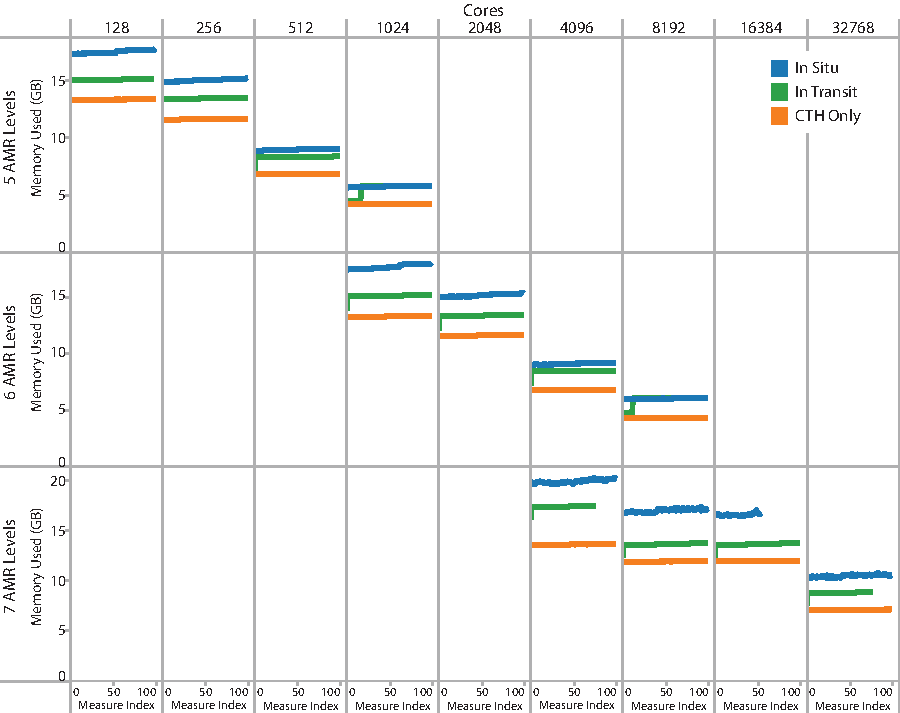
\includegraphics[width=\linewidth]{figures/MemoryUsageAll}
  \caption{Matrix of all measurements taken for memory usage comparisons.
    Each measurement is the total memory in use in a node (so for \insitu and
    \intransit memory includes both CTH simulation and overhead).  Each
    measurement is plotted as the maximum memory use in all nodes at the
    time the measurement was taken.}
  \label{fig:MemoryUsageAll}
\end{figure}

Figure~\ref{fig:MemoryInSituPerNode} gives a summary of the extra memory
used when using Catalyst for \insitu analysis during our experiments.
Likewise, Figure~\ref{fig:MemoryInTransitPerNode} gives the same summary
for the \intransit memory overhead for the nodes within the simulation
(memory usage on the separate analysis job is not given).  In all cases the
added overhead is less than 50\% than the memory used by CTH itself, and in
most cases the additional overhead is significantly smaller than that.

\begin{figure}[htb]
  \centering
  \includegraphics[width=\linewidth]{figures/MemoryUsageInSituPerNode}
  \caption{Plot of average per node memory usage of the \insitu run on Cielo.}
  \label{fig:MemoryInSituPerNode}
\end{figure}

\begin{figure}[htb]
  \centering
  \includegraphics[width=\linewidth]{figures/MemoryUsageInTransitPerNode}
  \caption{Plot of average per node memory usage of the \intransit run on Cielo.}
  \label{fig:MemoryInTransitPerNode}
\end{figure}

Figure~\ref{fig:MemoryCompare} compares the amount of memory per node added
when using \insitu versus \intransit.  As expected, the \intransit approach
requires a smaller memory overhead than \insitu within the nodes of the
simulation.  Thus, \intransit could be a better option when the simulation
requires as much memory per process as possible, but the \intransit
approach also requires separate nodes to be reserved for the analysis,
which also may cause the total amount of available simulation memory to be
reduced if nodes must be taken away from the simulation.

\begin{figure}[htb]
  \centering
  \includegraphics[width=\linewidth]{figures/MemoryUsageCompare}
  \caption{Plot of the average overhead per node of both \insitu and \intransit}
  \label{fig:MemoryCompare}
\end{figure}


